\documentclass[../main.tex]{subfiles}
\begin{document}
La cinematica studia il moto dei corpi, non le cause (quello fa parte della dinamica).

Il sistema di riferimento per la cinematica \textbf{unidimensionale} è composto da una sola retta, che possiamo definire a piacere:
\begin{center}
    \begin{tikzpicture}
         % Definizione dei vettori
        \draw[->, thick, black] (0,0) -- (5,0) node[midway, below] {$x$};

        \draw[->, thick, black] (-1,0) -- (-1,5) node[midway, below, left] {$y$};

        \draw[->, thick, black] (6,5) -- (6,0) node[midway, below, left] {$y$};
    \end{tikzpicture}
\end{center}

\begin{itemize}
    \item distanza $d \phantom{-} \lbrack m \rbrack$: lunghezza del percorso, sempre $\geq 0$
    \item spostamento $\Delta x$ oppure $\Delta y \phantom{-} \lbrack m\rbrack$: $\Delta x=x_f-x_i$: differenza di posizione
\end{itemize}
\textbf{Nota:} distanza $\neq$ spostamento, la distanza tiene conto del percorso e delle eventuali tappe, è un valore sempre positivo quindi anche se si torna indietro rispetto al sistema di riferimento aumenterà, lo spostamento invece è relativo soltanto a $x_i$ e $x_f$, non tiene conto di eventuali allungamenti di percorso, banalmente se torno mi muovo di 2 metri e ritorno al punto di partenza lo spostamento risulterà 0. Ecco alcuni esempi: \\ \\

\begin{center}
    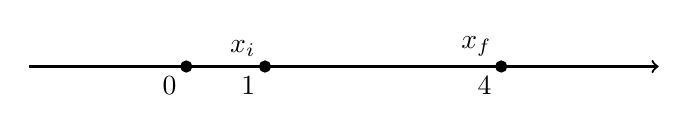
\begin{tikzpicture}
         % Disegna i punti
        \filldraw[black] (0,0) circle (2pt) node[anchor=north east] {0} ;
        \filldraw[black] (1,0) circle (2pt) node[anchor=north east] {1} node[anchor=south east] {$x_i$};
        \filldraw[black] (4,0) circle (2pt) node[anchor=north east] {4} node[anchor=south east] {$x_f$};

         % Definizione dei vettori
        \draw[->, thick, black] (-2,0) -- (6,0) node[midway, below] {};
    \end{tikzpicture}
    
    $d=3m\phantom{---} \Delta x=4-1=3m$
\end{center}
\vspace{0.5cm}
\begin{center}
    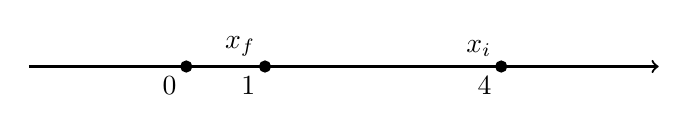
\begin{tikzpicture}
         % Disegna i punti
        \filldraw[black] (0,0) circle (2pt) node[anchor=north east] {0} ;
        \filldraw[black] (1,0) circle (2pt) node[anchor=north east] {1} node[anchor=south east] {$x_f$};
        \filldraw[black] (4,0) circle (2pt) node[anchor=north east] {4} node[anchor=south east] {$x_i$};

         % Definizione dei vettori
        \draw[->, thick, black] (-2,0) -- (6,0) node[midway, below] {};
    \end{tikzpicture}
    
    $d=3m\phantom{---} \Delta x=1-4=-3m$
\end{center}
\vspace{0.5cm}
\begin{center}
    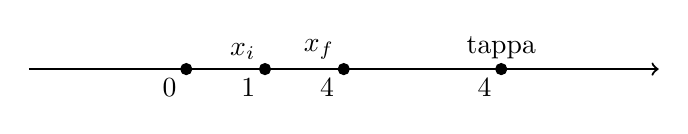
\begin{tikzpicture}
         % Disegna i punti
        \filldraw[black] (0,0) circle (2pt) node[anchor=north east] {0} ;
        \filldraw[black] (1,0) circle (2pt) node[anchor=north east] {1} node[anchor=south east] {$x_i$};
        \filldraw[black] (2,0) circle (2pt) node[anchor=north east] {4} node[anchor=south east] {$x_f$};
        \filldraw[black] (4,0) circle (2pt) node[anchor=north east] {4} node[anchor=south] {tappa};

         % Definizione dei vettori
        \draw[->, thick, black] (-2,0) -- (6,0) node[midway, below] {};
    \end{tikzpicture}
    
    $d=3+2=5m\phantom{---} \Delta x=2-1=1m$
\end{center}
\vspace{0.5cm}
\begin{itemize}
    \item velocità scalare media $v=\frac{d}{t} \phantom{-} \lbrack \frac{m}{s}\rbrack$: lunghezza del percorso, sempre $\geq 0$
    \item velocità media $v=\frac{\Delta x}{\Delta t} \phantom{-}\lbrack \frac{m}{s}\rbrack$: può essere negativa \begin{align*}
        v&=\frac{x_f-x_i}{t_f-t_i} \\
        &=\frac{x_f-x_i}{t} \text{ con } t_i=0s
    \end{align*}
    \item velocità istantanea $v_i=\lim\limits_{\Delta t \to 0}\frac{\Delta x}{\Delta t}$
\end{itemize}
\textbf{Nota:} nella velocità istantanea $\Delta t$ è tendente a 0, si calcola quindi la pendenza della retta tangente (la formula è uguale a quella della velocità media solo che $\Delta t$ tende a $0$.


\end{document}